\documentclass[10pt,a4paper]{article}
\usepackage[utf8]{inputenc}
\usepackage{amsmath}
\usepackage{amsfonts}
\usepackage{amssymb}
\usepackage{graphicx}
\usepackage[left=2cm,right=2cm,top=2cm,bottom=2cm]{geometry}
\author{Gabriel Alvarez Sotelo
Ing Mecatronica
carlos moran garabito
sistemas electronicos de interfaz}
\title{Operacion de los circuitos de activacion con tiristores en convetidores CA-CD y CA-CA}
\begin{document}
\maketitle\

\includegraphics[width=18cm]{latex/upzmg.jpeg} 
\newpage
\maketitle\section{Convertidor CA-CD ¿para que sirve?}
Un  convertidor  de  corriente  alterna  a  corriente  directa  parte  de  un  rectificador  de  onda  completa,  Su  carga  puede  ser  puramente  resistiva y al  agregarle  a  este  rectificador  un  capacitor en paralelo el convertidor se comporta como un filtro ya que se produce un voltaje a la salida que es esencialmente continuo,el  convertidor  CA-CD  nos  proporciona  una  señal  de  salida  rectificada que casi es constante con el valor  Vm,  donde  Vm  es  igual  al  valor  pico  del  voltaje  de  entrada como este  voltaje  casi  constante  presenta  una  variación  de  V0.  Este  valor  se  puede  considerar  muy  pequeño  y  de  esta  manera  encontrar  el  valor  del  resistor  y  del capacitor para un valor de voltaje directo deseado. 



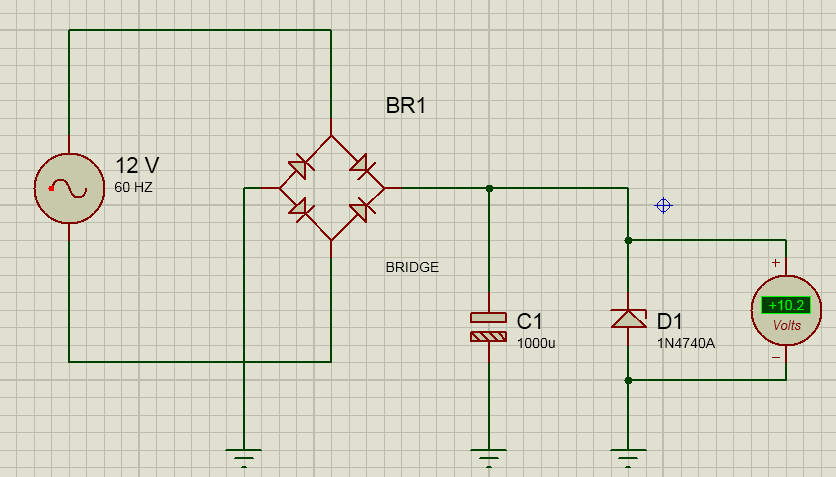
\includegraphics[width=10cm]{latex/caycd.png} 
\maketitle\section{Convertidor CA-CA ¿para que sirve?}
Los convertidores CA a CA estan destinados a controlar el flujo de corriente alterna mediante la variacion del valor aficaz (RMS) el voltaje de CA aplicado ala carga, y que la frecuencia de salida de estos convertidores es la misma frecuencia del vltaje de su reespectiva entrada.
a estos tambien se les puede conocer como "controladores del voltaje de CA ya que estos tienen aplicacion de de calefaccion industrial, cambio de conexiones con transformadores con carga, controles de alumbrado.

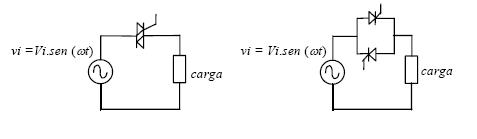
\includegraphics[width=18cm]{latex/circuito.jpg} 
\newpage



\maketitle\section{Operacion de los circuitos de activacion con tiristores}
Los  convertidores  de  corriente  directa  a  corriente  alterna  son  utilizados  como  drivers  de  motores  y  como  fuentes  de  corriente  alterna  ininterrumpida  y  tienen  como  objetivo  producir  una  señal  de  corriente  alterna  sinusoidal,  cuya  magnitud  y  frecuencia  puedan  ser  controladas ya que existen  diversos  tipos  de  convertidores  inversores  de  los  cuales  el  convertidor  de  una  sola  pierna  y  el  convertidor  en  puente  de  media  y  onda  completa, estas  topologías  generan  una  señal  de  salida  que  oscila  entre  el  valor  constante  +Vd/2  y  –Vd/2 para medio puente y una sola pierna, y +Vd y –Vd  para puente completo,todo esto a pesar  de  que  esta  señal  es  cuadrada,  posteriormente  se  filtra  para  obtener  una  señal  senoidal.


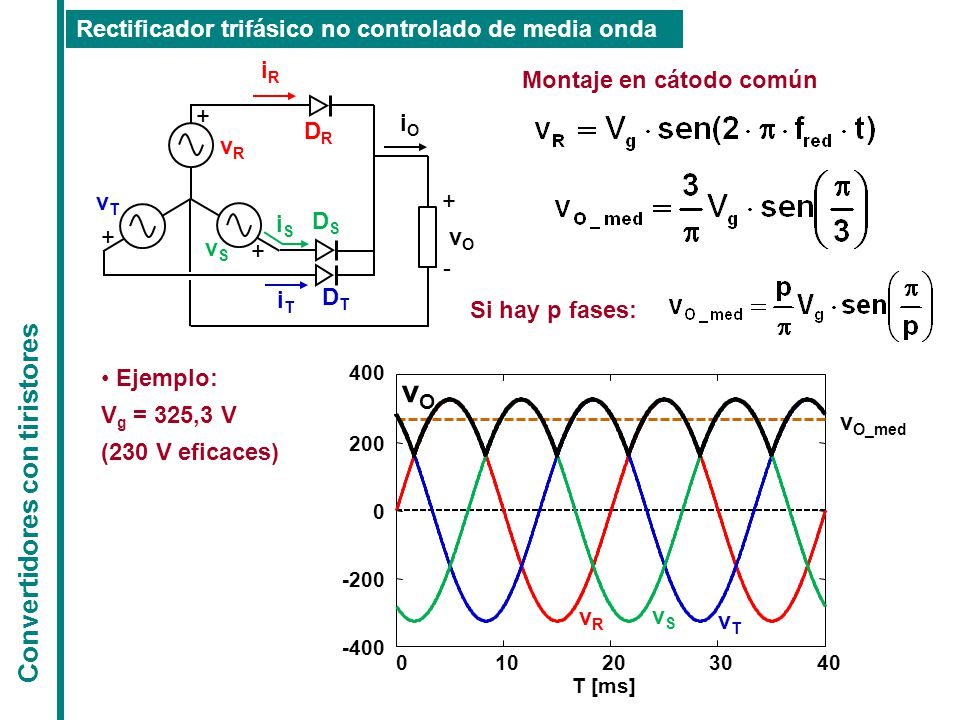
\includegraphics[width=18cm]{latex/rectificador.jpg} 



 
\end{document}